\section{Systeemarchitectuur}
Dit hoofdstuk beschrijft de architectuur van het Smart Markers systeem.

\subsection{Architectuur}
De netwerkarchitectuur heeft een stertopologie, waarin de LoRa gateway centraal staat. De GPS-nodes, die om de gateway en over een gebied zijn verspreid, sturen GPS-data naar de gateway. Van één van de GPS-nodes is de positie nauwkeurig opgemeten, deze node functioneert als referentiestation en stuurt GPS-correctiedata naar de gateway. De gateway stuurt deze data door naar een applicatieserver, waar de GPS-data en de GPS-correctiedata worden gebruikt om de GPS-data tot op een meter nauwkeurig te krijgen.

In hoofdstuk \ref{subsec:overzicht} staat een schematisch overzicht van de Smart Markers architectuur.

\subsection{Hardware}
\paragraph{STM32 microcontroller}
Als brein van de Smart Marker is er gekozen voor een \texttt{STM32 NUCLEO-L073RZ development board}, omdat het board:
\begin{itemize}
    \item beschikt over een ARM Cortex M0+ 32 bit processor;
    \item beschikt over voldoende geheugen voor de Smart Marker applicatie;
    \item weinig energie verbruikt;
    \item zich leent voor prototyping;
    \item een veelgebruikte en bekende architectuur heeft;
\end{itemize}

\paragraph{LoRa radio}
De LoRa radio bevindt zich op het RF-LORA-868-SO board. De SX1272 LoRa radio wordt voornamelijk gebruikt voor end-devices, omdat het een half-duplex radio is.
% TODO: Links naar LoRa docs

\paragraph{GPS-modules}
Voor de locatiebepaling worden u-blox EVK-7P GPS-modules gebruikt, omdat Kadaster deze heeft aangeboden voor gebruik tijdens dit project. GPS-modules zijn relatief duur, dus qua budget komt het goed uit dat Kadaster deze modules ter beschikking kan stellen.

Deze GPS-modules worden uitgelezen over de SPI-bus, met een maximale snelheid van 1Mb/s. Er zijn twee protocollen voor de representatie van de output data: het UBX-protocol voor binaire representatie en het NMEA-protocol voor ASCII representatie.
% TODO: Meer onderzoeken. Welke data?

\paragraph{Stroomvoorziening}
Als energiebron gebruiken we twee 18650 cellen, welke extern opgeladen worden.
Om te voorkomen dat deze te ver ontladen worden zal hier een bescherming voor
ingebouwd worden. Voorlopig zullen de cellen extern geladen worden, in een meer
definitieve versie zal het laden geïntegreerd kunnen worden.

\subsection{Software}
Tijdens het project wordt er gebruik gemaakt van softwarepakketten ter ondersteuning. Hieronder staat een korte opsomming van tools en technieken die tijdens het project worden gebruikt:
\begin{itemize}
    \item GNU ARM embedded toolchain;
    \item Makefiles;
    \item ST-Link programmer;
    \item Git;
    \item \LaTeX;
\end{itemize}

\subsection{Communicatie}
Als communicatie techniek is er gekozen voor LoRa, omdat de opdrachtgever met één meting een heel gebied wilt kunnen registreren. De LoRa modulatietechniek leent zich ervoor om in deze use-case gebruikt te worden, vanwege de lange communicatie-afstand en het lage energieverbruik.

Er is overwogen om een LoRa mesh netwerk op te zetten, echter is er besloten om te kiezen voor een simpelere implementatie, vanwege de korte tijdsduur van het project en een gebrek aan kennis over mesh netwerken. Uit het onderzoek van \citep{AIM_HI_LORA_WMN} is gebleken dat de packet delivery ratio (PDR) in hun labopstelling aanzienlijk betere resultaten had in een mesh netwerk (, ten opzichte van een stertopologie.

\subsection{Gegevensopslag}
De verzamelde data uit de meetpunten zal worden opgeslagen in een SQL-database.
Zie ook hoofdstuk \ref{sec:database}.

\label{subsec:overzicht}
\subsection{Overzicht}
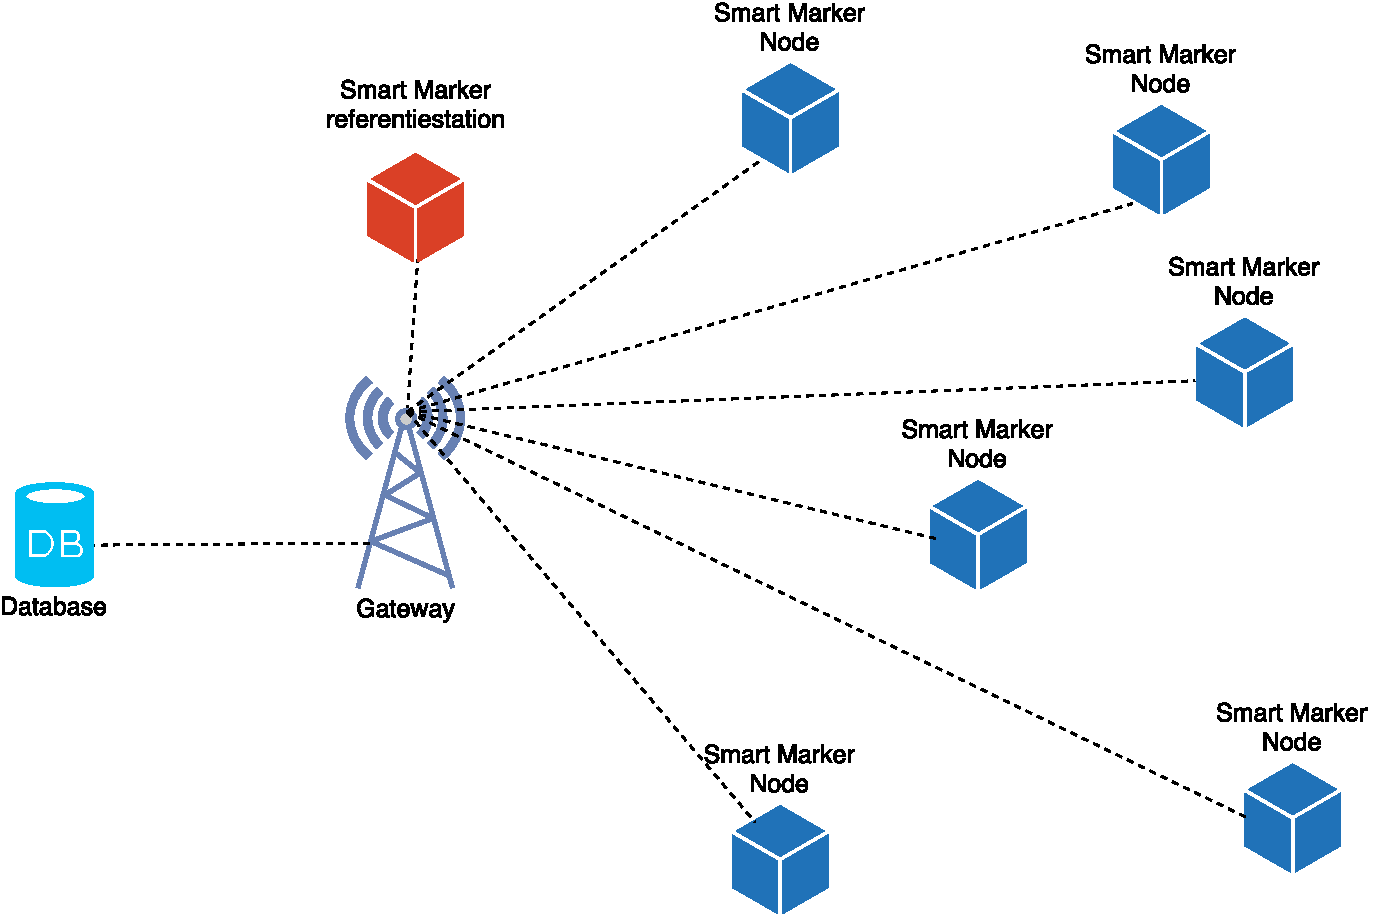
\includegraphics[width=0.9\linewidth]{technical/system_architecture_overview.pdf}
